% Reparametrization: beta = alpha o h has the same trace as alpha (compare Fig. 10 of Delgado and Frensel).
% Build the SVG with ./build.sh (needs latex and dvisvgm, both part of MacTeX).
\def\pgfsysdriver{pgfsys-dvisvgm.def}
\documentclass[tikz,border=6pt]{standalone}
\usepackage{amsmath,amssymb}
\usetikzlibrary{calc}
\definecolor{curve}{HTML}{2563EB}
\definecolor{pt}{HTML}{D97706}
\definecolor{ink}{HTML}{1C1F26}
\definecolor{soft}{HTML}{6B7280}
\definecolor{green}{HTML}{16A34A}
\begin{document}
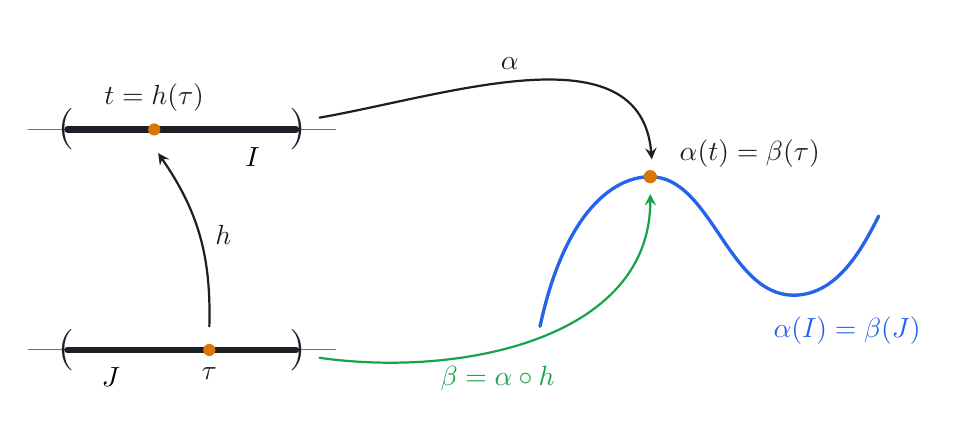
\begin{tikzpicture}[>=stealth, line cap=round, line join=round]
  % the interval J and the parameter tau
  \draw[soft] (-0.3,0) -- (3.6,0);
  \draw[line width=2.4pt, ink] (0.2,0) -- (3.1,0);
  \node[ink, scale=1.5] at (0.18,0) {(};
  \node[ink, scale=1.5] at (3.12,0) {)};
  \node[below=3pt] at (0.75,0) {$J$};
  \fill[pt] (2.0,0) circle (2.2pt) node[below=3pt, ink] {$\tau$};

  % the interval I and the parameter t = h(tau)
  \draw[soft] (-0.3,2.8) -- (3.6,2.8);
  \draw[line width=2.4pt, ink] (0.2,2.8) -- (3.1,2.8);
  \node[ink, scale=1.5] at (0.18,2.8) {(};
  \node[ink, scale=1.5] at (3.12,2.8) {)};
  \node[below=3pt] at (2.55,2.8) {$I$};
  \fill[pt] (1.3,2.8) circle (2.2pt) node[above=3pt, ink] {$t=h(\tau)$};

  % h : J -> I
  \draw[->, thick, ink] (2.0,0.3) to[bend right=18] node[right=2pt] {$h$} (1.35,2.5);

  % the trace
  \begin{scope}[shift={(6.2,0.1)}]
    \draw[very thick, curve] (0,0.2) .. controls (0.3,1.6) and (0.9,2.1) .. (1.4,2.1)
                             .. controls (2.2,2.1) and (2.4,0.5) .. (3.3,0.6)
                             .. controls (3.8,0.65) and (4.1,1.2) .. (4.3,1.6);
    \coordinate (Q) at (1.4,2.1);
    \node[curve] at (3.9,0.15) {$\alpha(I)=\beta(J)$};
  \end{scope}

  % alpha : I -> R^2 and beta = alpha o h : J -> R^2
  \draw[->, thick, ink] (3.4,2.95) to[out=10, in=95] node[above=1pt, pos=0.45] {$\alpha$} ($(Q)+(0.02,0.22)$);
  \draw[->, thick, green] (3.4,-0.1) to[out=-8, in=-90] node[below=2pt, pos=0.4] {$\beta=\alpha\circ h$} ($(Q)+(0,-0.22)$);
  \fill[pt] (Q) circle (2.4pt);
  \node[ink, anchor=west] at ($(Q)+(0.25,0.3)$) {$\alpha(t)=\beta(\tau)$};
\end{tikzpicture}
\end{document}
